\section{Introduction}
\label{sec:Int}

This section presents the research design for the project \emph{Minimal, Resource-Bounded Runtime Verification for a Safety-Critical Automotive ECU}. It follows the structure of the Research Design II write-up, covering the theme and rationale, research positioning, background, hypothesis, and the overall aim and purpose of the study.

\subsection{Title and Programme Details}

\textbf{Module:} MCAST IICT -- Research Design II (2025/2026)

\textbf{Student:} Damian Navarro

\textbf{Programme:} BSc (Hons) Software Development

\textbf{Institute:} Institute of Information and Communication Technology (IICT), MCAST

\subsection{Chosen Research}

The working title of the research is:

\begin{quote}
Minimal, Resource-Bounded Runtime Verification for a Safety-Critical Automotive ECU.
\end{quote}

The design is grounded in recent work on \textbf{automotive cybersecurity testing}, \textbf{runtime verification for CPS/IoT}, and \textbf{hardware-anchored trust and attestation}~\cite{ekert2021cybersecurity,zhang2024context,dehoz2022iotdt,plappert2023hta}.

\subsection{Theme and Topic Rationale}

\textbf{Theme:} Safety and cybersecurity assurance for cyber-physical and IoT-like automotive systems.

\textbf{Specific topic:} Designing a minimal set of runtime monitors for a safety-critical ECU (e.g.\ braking), implementable on constrained hardware while supporting current automotive cybersecurity and homologation requirements~\cite{ekert2021cybersecurity,krichen2023survey}.

\textbf{Rationale:} New vehicles contain many real-time ECUs connected via CAN-FD buses and a central gateway, and must pass large cybersecurity verification and validation (V\&V) test suites under norms such as SAE J3061 and ISO 21434 for homologation~\cite{ekert2021cybersecurity}. At the same time, IoT-class and automotive controllers are constrained in CPU, memory, power, and area, which limits the applicability of heavyweight security and verification mechanisms~\cite{williams2022survey,saadat2024rosmonitoring2}.

Formal verification and validation surveys for IoT highlight scalability and state-explosion challenges, and recommend lightweight, runtime-oriented approaches for safety- and security-critical systems~\cite{krichen2023survey}. Runtime verification (RV) has been shown to be a \textbf{pragmatic} technique for CPS and automotive domains, where specifications are represented as automata and monitored during execution~\cite{zhang2024context,dehoz2022iotdt}. An IoT digital-twin approach demonstrates that only a subset of network traffic needs monitoring to detect communication violations, achieving negligible overhead on constrained devices~\cite{dehoz2022iotdt}.

To protect keys, firmware, and measurements on resource-constrained platforms, work on hardware trust anchors and remote attestation shows how hardware-based roots of trust and hybrid attestation protocols can provide integrity guarantees while preserving availability~\cite{saadat2024rosmonitoring2,plappert2023hta}.

This motivates exploring \textbf{how to specify and embed a small, local runtime monitor on a safety-critical ECU} that respects strict resource and timing constraints while contributing to cybersecurity and safety assurance.

\subsection{Positioning and Research Onion}

\begin{figure}[ht]
  \centering
  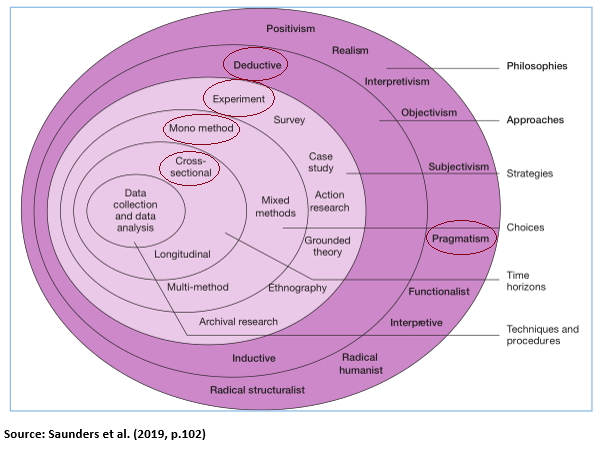
\includegraphics[width=\columnwidth]{../figure-1-research-onion.png}
  \caption{The research onion (adapted from Saunders \textit{et al.})~\cite{saunders2016research}.}
  \label{fig:research-onion}
\end{figure}

This study investigates a minimal, resource-bounded runtime verification mechanism for a safety-critical automotive Electronic Control Unit (ECU) using a simulation-based experimental design. The methodology is structured according to the layers of the Saunders \textit{et al.} research onion~\cite{saunders2016research}.

\paragraph{Research Philosophy: Pragmatism.}
The research is grounded in a \textbf{pragmatist} philosophy, focusing on developing a solution that is practically effective under realistic resource constraints. The value of the work is judged by whether the proposed runtime verification approach can be integrated into an automotive ECU context and meet performance and safety requirements, rather than by commitment to a single ontological or epistemological stance.

\paragraph{Research Approach: Deductive.}
A \textbf{deductive} approach is adopted. Existing theory and prior work on runtime verification, safety-critical systems, and real-time resource constraints are used to derive expectations about the behaviour of a minimal monitoring mechanism (e.g., that it should incur low overhead while reliably detecting property violations). These theoretically informed expectations are then tested empirically through controlled experiments in a simulated ECU environment.

\paragraph{Methodological Choice: Quantitative Mono Method.}
The study employs a \textbf{quantitative mono-method} design. All primary data are numerical, capturing performance and correctness characteristics of the monitored system. Key variables include execution time overhead, CPU utilisation, memory footprint, and the rate of correctly detected versus missed property violations. These quantitative measures form the basis for assessing whether the proposed mechanism satisfies the targeted resource bounds and safety criteria.

\paragraph{Research Strategy: Experiment.}
The chosen research strategy is an \textbf{experiment}. A runtime verification component is implemented and integrated with a simulated model of a safety-critical automotive ECU. Experimental runs are conducted under controlled conditions, where input workloads, operating scenarios, and injected faults are systematically varied. A baseline configuration without monitoring is used for comparison, enabling the isolation of the effects of the runtime verification mechanism on system performance and fault detection.

\paragraph{Time Horizon: Cross-Sectional.}
The research adopts a \textbf{cross-sectional} time horizon. Data are collected during a finite experimental campaign consisting of multiple simulation runs, each representing a distinct configuration or scenario. The study does not follow the system over an extended real-world operational period; instead, it captures system behaviour at a specific point in time under a range of controlled experimental conditions.

\paragraph{Data Collection and Analysis Procedures.}
Data collection is performed by instrumenting the simulated ECU environment to record, for each run: cycle-level execution time, CPU load, memory usage attributable to the monitoring component, and whether injected property violations are detected or missed. Faults are injected into the simulated system (for example, by altering parameters or timing) to evaluate the effectiveness of the runtime verification mechanism.

The collected data are analysed using descriptive statistics (such as means and variances of overhead metrics) and comparative analysis between the monitored and unmonitored configurations. This analysis quantifies the performance impact of the monitoring mechanism and its detection capabilities relative to the derived requirements. The results are then interpreted in light of the research objectives to determine whether the minimal, resource-bounded runtime verification approach is suitable for deployment in safety-critical automotive ECU settings.

\subsection{Background to the Research Theme}

Modern vehicles are complex cyber-physical systems with many ECUs and a central gateway; cybersecurity V\&V must cover thousands of network-level test cases to satisfy norms like ISO 21434, influencing how in-vehicle communication is tested and which attack patterns are considered before road release~\cite{ekert2021cybersecurity}. Parallel developments in IoT show that pervasive connectivity increases the attack surface, while device constraints hinder deployment of traditional security mechanisms~\cite{williams2022survey}.

Formal verification and validation surveys for IoT systems emphasise that exhaustive techniques often do not scale, and advocate combining formal specification with lightweight testing and runtime techniques~\cite{krichen2023survey}. In intelligent transport and autonomous vehicles, automata-theoretic, context-aware runtime monitors have been shown to detect unsafe events under varying environmental conditions by composing environment models with system B\"uchi automata~\cite{zhang2024context}.

For IoT communications, a digital-twin-based security architecture uses rule-based runtime verification of parametric events (packets) and demonstrates that monitoring only a subset of traffic can still detect protocol violations with negligible overhead on limited devices~\cite{dehoz2022iotdt}. Runtime verification has also been generalised in an algebraic framework that views runs and specification automata through monoidal and semiring structures, enabling incremental, quantitative monitoring and case studies in the automotive domain~\cite{jaksic2018algebraic}.

On the trust side, surveys of IoT security and remote attestation underline the importance of offloading verification to more capable entities while providing device integrity proofs, especially when local resources are scarce~\cite{williams2022survey,saadat2024rosmonitoring2}. Hybrid remote attestation protocols specifically target IoT devices, combining randomised memory checks with physical unclonable functions to achieve high availability and low energy usage~\cite{plappert2023hta}. Evaluations of hardware trust anchors for automotive applications compare different HTA designs against current and emerging automotive requirements, and identify options that are feasible even for highly constrained controllers~\cite{plappert2023hta}.

This body of work collectively supports investigating a \textbf{minimal, resource-bounded runtime verification design} for a safety-critical ECU that:
\begin{itemize}
  \item aligns with automotive cybersecurity test practice and regulation~\cite{ekert2021cybersecurity},
  \item leverages lightweight RV techniques proven in CPS and IoT contexts~\cite{krichen2023survey,zhang2024context,dehoz2022iotdt}, and
  \item is protected and supported by hardware-anchored trust and remote attestation mechanisms~\cite{saadat2024rosmonitoring2,plappert2023hta}.
\end{itemize}

\subsection{Hypothesis}

A carefully selected, minimal set of local safety and security properties for a safety-critical automotive ECU can be implemented as runtime monitors with bounded time and memory overhead such that:

\begin{itemize}
  \item they detect violations relevant to automotive cybersecurity and safety requirements~\cite{ekert2021cybersecurity,krichen2023survey,zhang2024context,dehoz2022iotdt,lorych2024hta}, and
  \item they remain compatible with the resource and availability constraints of in-vehicle and IoT-class controllers~\cite{williams2022survey,saadat2024rosmonitoring2,plappert2023hta}.
\end{itemize}

Formally:

\begin{quote}
\textbf{H\textsubscript{1}:} Minimal, local runtime monitors for a safety-critical ECU can provide meaningful safety and cybersecurity coverage without violating the ECU's real-time and resource constraints.
\end{quote}

\subsection{Research Aim and Purpose}

\textbf{Aim:} To design and analytically evaluate a minimal, resource-bounded runtime verification monitor for a safety-critical automotive ECU, drawing on automotive cybersecurity V\&V practice, CPS/IoT runtime verification techniques, and hardware-anchored trust and attestation mechanisms~\cite{ekert2021cybersecurity,zhang2024context,dehoz2022iotdt,lorych2024hta,saadat2024rosmonitoring2,plappert2023hta}.

\textbf{Purpose:}
\begin{itemize}
  \item To derive a method for selecting and formalising a small set of ECU-local properties as automata or algebraic specifications suitable for runtime monitoring under tight resource constraints~\cite{krichen2023survey,zhang2024context,dehoz2022iotdt}.
  \item To propose an integration strategy that minimises monitoring overhead through selective observation of events/messages, while still addressing key cybersecurity and safety requirements~\cite{ekert2021cybersecurity,krichen2023survey,zhang2024context,dehoz2022iotdt,lorych2024hta}.
  \item To outline how hardware trust anchors and remote/hybrid attestation can protect the monitor and its artefacts in automotive-grade, resource-constrained environments~\cite{williams2022survey,saadat2024rosmonitoring2,plappert2023hta}.
\end{itemize}

This provides a focused design blueprint that can later be extended and evaluated in broader connected-vehicle and IoT security architectures.